%!TEX root=../tax-democracy-held.tex
%TODO rewrite abstract
%This is context (says art):
%TODO there is a better, more standard version of this in fishkin branch
I wonder:\cite{}
why, in the richest of countries, in the most enlightened of times (current day \gls{oecd}-world), are our welfare states so constrained and inefficient, our democracies so confused and distorted?
	%do I mean something specific/scientific by these adjectives?
	%you should cite some previous author, literature on here (you'll pick your reviewer!, also, you really need to give credit! says Art).
	%say what you're problem is with the mainstream literature.
	%Don't say criticize.
	%So far, this question has been answered by looking at welfare state spending and revenue. %However, \ldots
	%However, this work would benefit from alternative configurations of welfare states and democracies, and for failing to explain their absence. %put something equally concrete as spending and revenue, examine the tax law itself.
	%explain welfare state retrenchment
	%include the whole progression thing earlier
	%stress that this is an experiment, which isn't so common otherwise (this would make it sexy) (include control groups)
	%maybe include the questionnaire, do pre/post, 4-5 days,
	%absolutely stress the sense of validity
I ask:
if a hypothetical, superior political process (deliberative democracy) ruled our polity, would we think better and fairer about the institutions of the mixed economy and would we opt for a hypothetical, superior tax regime (\gls{pct}, \gls{lvt} and \gls{nit})?
%comment MN: is it?

And so I test:
if given the possibility to deliberate well-informed, fairly and thoroughly (a deliberative forum), will randomly selected, ordinary voters understand the mixed economy differently (better) and prefer a different tax (\gls{pct}, \gls{lvt} and \gls{nit})?
%control group

	%We hope that people will understand and prefer [use same concepts as above, link] a more progressive and efficient tax

If, in fact, they do, welfare state research will have a lot more to explain, and deliberative democracy will have shown its stripes.

%\begin{figure}[htbp]
%	\centering
%	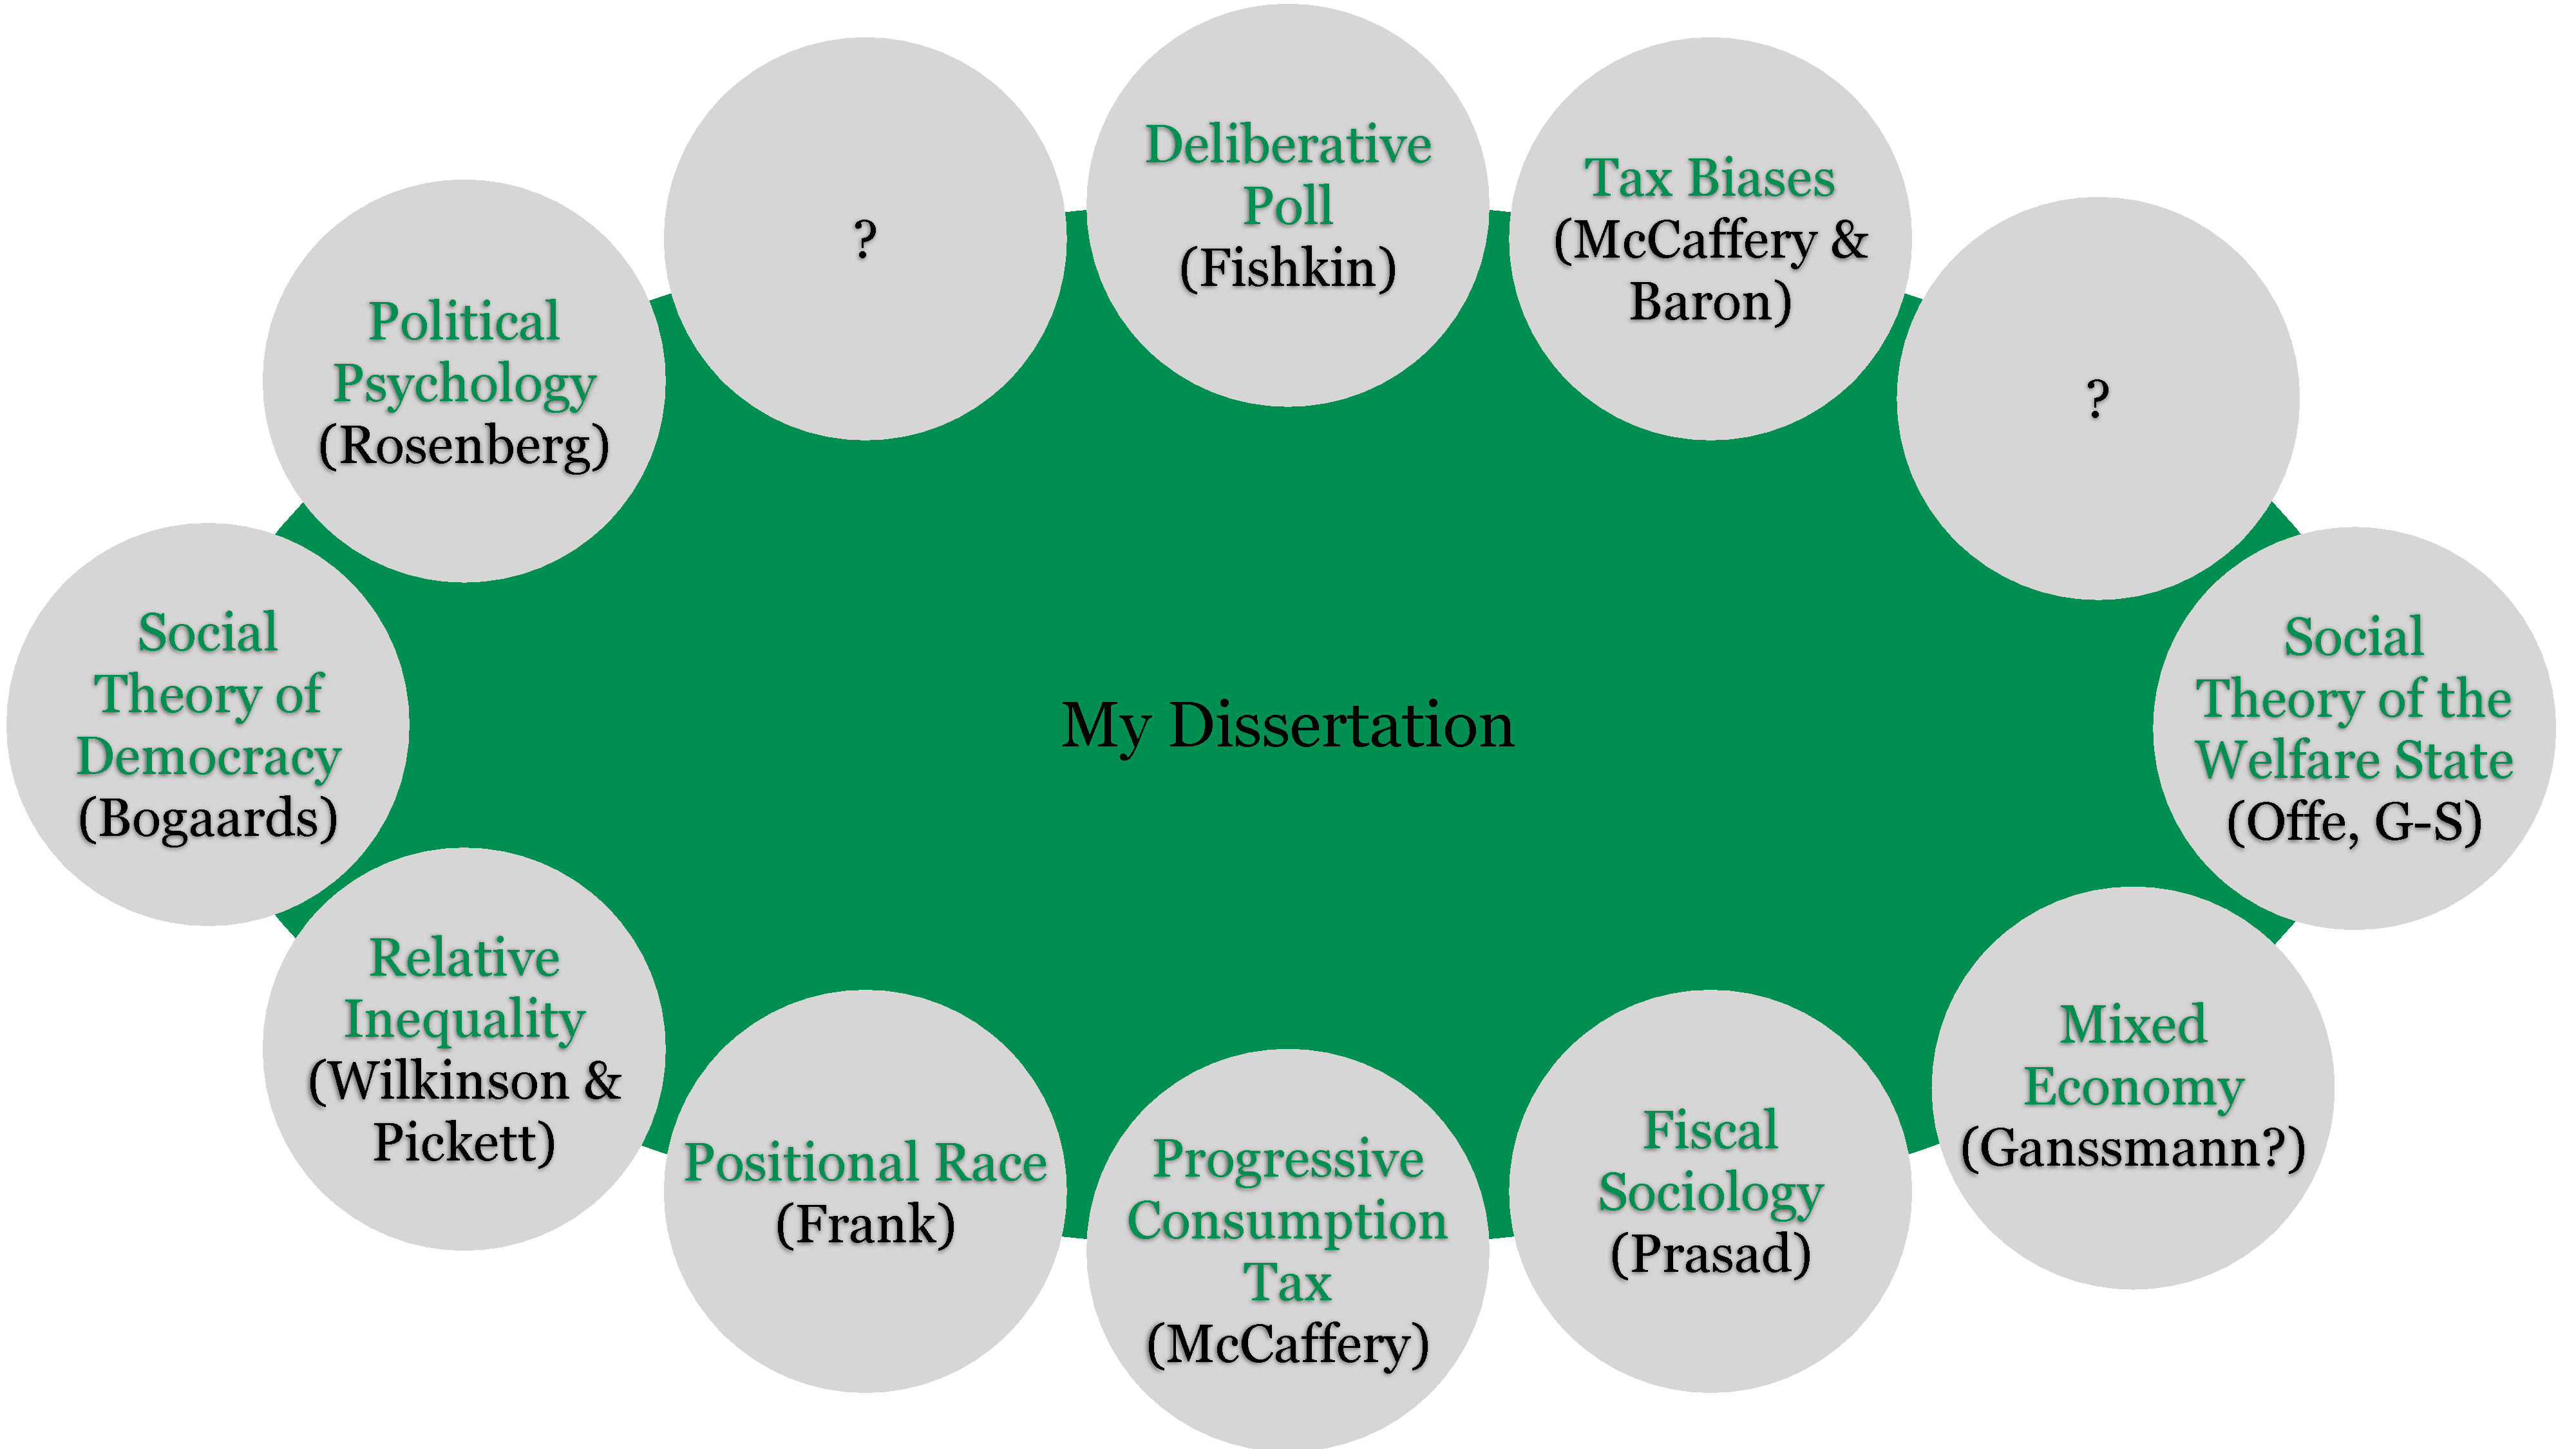
\includegraphics[width=1\linewidth]{diss-expertise}
%	\caption{Academic Fields and Advisors for this Dissertation}
%	\label{fig:diss-expertise}
%\end{figure}
%
%\begin{landscape}
%\begin{figure}[htbp]
%	\centering
%	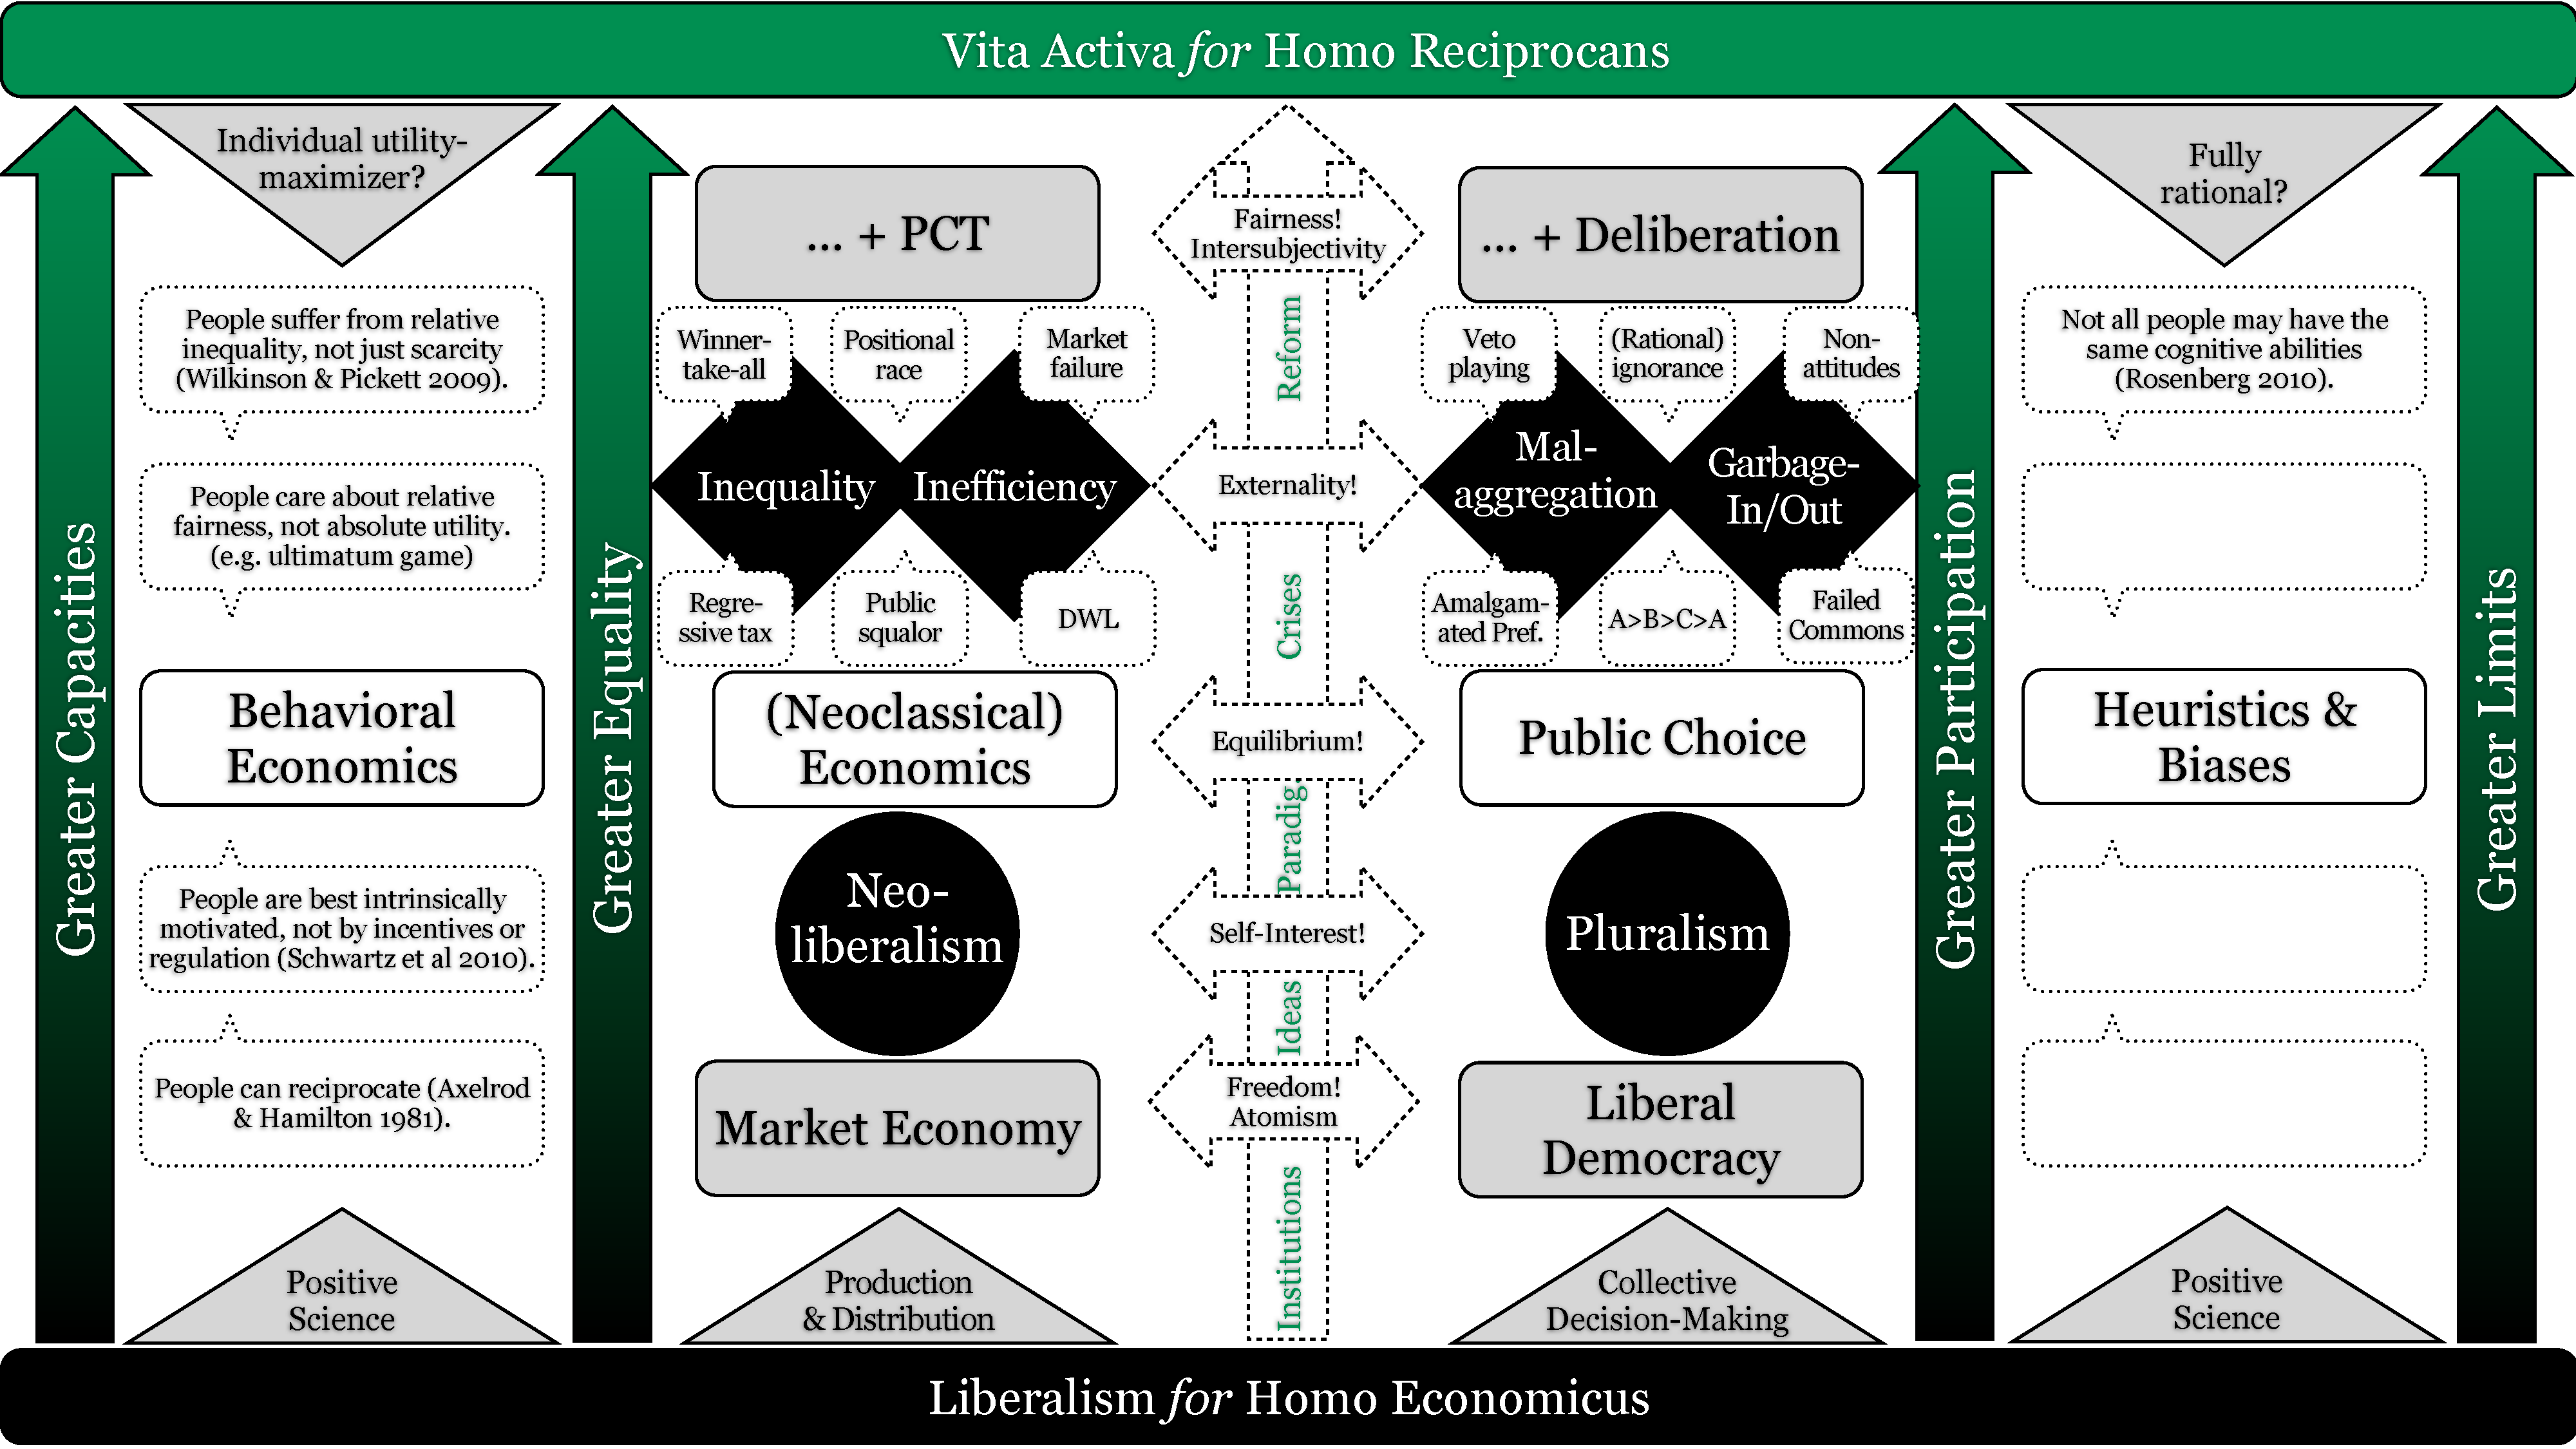
\includegraphics[width=1\linewidth]{diss-mindmap}
%	\caption{Mindmap of this Dissertation}
%	\label{fig:diss-mindmap}
%\end{figure}
%\end{landscape}

%comment MN: zwei sehr starke apriori annahmen
	%1 überlegegenes demokratisches Verfahren, politisches verfahren
	%2 überleges steuersystem
	%Aber: Ratio UND Emotion, Argument UND Narration, Gemein UND Eigeninteresse. Wieso priviligierung *eines* Pols?

As capitalism matures, commerce globalizes and inequalities widen, the mixed economies of the Organisation for Economic Co-Operation and De- velopment (OECD) face steeper tradeoffs between e


As capitalism matures, commerce globalizes and inequalities widen, the mixed economies of the Organisation for Economic Co-Operation and De- velopment (OECD) face steeper tradeoffs between efficiency, equity and sus- tainability in taxation.
Suboptimal taxation of (some) incomes and postpaid consumption undermines state-market balances, retrenches welfare and, ul- timately, constrains democratic rule of the economy.
Progressive taxation of consumption defined as income minus net savings (Progressive Consumption Tax (PCT)) or rent capture on natural resources and unimproved land value (Land Value Tax (LVT)) appear to or higher tradeo↵s, but remain hypothetical and are hardly discussed in science or the public.
Similarly, as complexity increases, special interests concentrate and traditional alle- giances wane, the liberal democracies of the OECD face steeper tradeoffs between mass participation, political equality and enlightened understand- ing.
Representative, pluralist democracy suffrs from resultant malaggregations and ill-formed preferences, and, ultimately, impairs political equality in the face of economic inequality.
Collective decisions by ordinary citizens, based on mutual respect, balanced information and reason-giving promise to better uphold liberal democracy, but such deliberation has hardly been tried on abstract and complex choices.
I here propose to investigate whether, and how, people can deliberate an issue as complex and pervasive as tax, and, conversely, whether, and how people change their beliefs and preferences about taxation as a result of such deliberation.
To test this, I invite a diverse sample of around 80 Bremen-areacitizenstoparticipateinadaylongDeliberativePoll in which they discuss basic choices in tax base and schedule in moderated small-group and plenary sessions.
Participants will receive a balanced brief- ing book and have access to a diverse panel of experts.
I will quantitatively compare participants’ responses to closed-ended questionnaires handed out before and after the event.
In addition, I will qualitatively compare selec- tively transcribed recordings of participants’ deliberations with arguments and concepts broadly consensual among economists.
I may further subject some groups to short learning interventions, targeted at improving partici- pant understanding of select concepts and abstractions deemed relevant for an informed choice of base and schedule.
If ordinary citizens can be shown to competently deliberate an issue as demanding as taxation, deliberative democrats will have more reason to be confident in their procedures and standards.
If ordinary citizens can be shown to prefer different tax bases and schedules as a function of greater knowledge and deliberation, welfare state research and political economy will have to explain the absence of such a morally relevant hypothetical.

Why,

Deliberative democracy from the first [CiviCon Citizen Conference](http://www.civicon.de) in 2014, where fifteen
I present **evidence** from the

I wonder:
why, in the richest of countries, in the most enlightened of times (current day OECD-world), are our welfare states so constrained and inefficient, our democracies so confused and distorted?

I ask:
if a hypothetical, superior political process (deliberative democracy) ruled our polity, would we think better and fairer about the institutions of the mixed economy and would we opt for a hypothetical, superior tax regime (PCT, LVT, NIT)?

And so I test:
if given the possibility to deliberate well-informed, fairly and thoroughly (a deliberative forum), will randomly selected, ordinary voters understand the mixed economy differently (better) and prefer a different tax (PCT, LVT, NIT)?

I present evidence from the first [CiviCon Citzen Conference](http://www.civicon.de) in 2014, where 16 ordin

If, in fact, they do, welfare state research will have a lot more to explain, and deliberative democracy will have shown its stripes.
